\subsection {An\'alisis de ECM y PSNR}

En el trabajo medimos la calidad de los m\'etodos para hacer una c\'amara lenta
de los videos bajando algunos videos con diferentes propiedades de internet
(osea que tienen relevancia en el mundo real), y sacando todos los frames
excepto uno de cada $c$. Luego se aplica alguno de los m\'etodos para generar un
video nuevo, con la misma cantidad de frames que el video original, que
idealmente ser\'ia igual (aunque es matem\'aticamente imposible \footnote{por el
principio del palomar} que haya un m\'etodo perfecto para todos los videos).

Luego, para medir el error entre el nuevo video en c\'amara lenta y el video
original se usa uno de dos m\'etodos: el \textbf{Error Cuadr\'atico Medio} o ECM
y el \textbf{Peak Signal to Nouse Ratio} o PSNR, que se definen como

\[
ECM(F, \bar{F}) = \frac{1}{m n} \sum^m_{i = i} \sum^n_{j = 1} \left| F_{k_{i j}} - \bar{F}_{k_{i j}} \right|^2
\]
\[
PSNR(F, \bar{F}) = 10 \; log_{10} \left( \frac{255^2}{ECM(F, \bar{F}} \right)
\]

Con $n$ igual a la altura de la im\'agen y $m$ igual a su largo. Estos dos
valores son importantes ya que, aunque los m\'etodos trabajen
``individualmente'' en un solo pixel, y el resultado de estos ser\'ian lo mismo
corriendose en mismo video que individualmente, ya que las pruebas son con videos
reales.

Hicimos los an\'alisis sobre 3 de los videos que contenian propiedades
interesantes: \textit{camerachanges.mp4}, \textit{slowmovescene.mp4}, y
\textit{funnybaby.avi}, y sobre los tres algoritmos. Como los videos son
relativamente peque\~nos y, por ende, el m\'etodo de splines es r\'apido,
dejamos el parametro $r$ del m\'etodo, que controla cada cuantos frames se
vuelven a empezar los splines, igual a $\infty$, osea que se hace un solo spline
para cada pixel del video.

Para ver como se comportaban los algoritmos mediante en salto, medimos el
\textbf{ECM} para saltos de 1, 3, 5, 7, y 10 frames:

\begin{figure}[H]
\centering
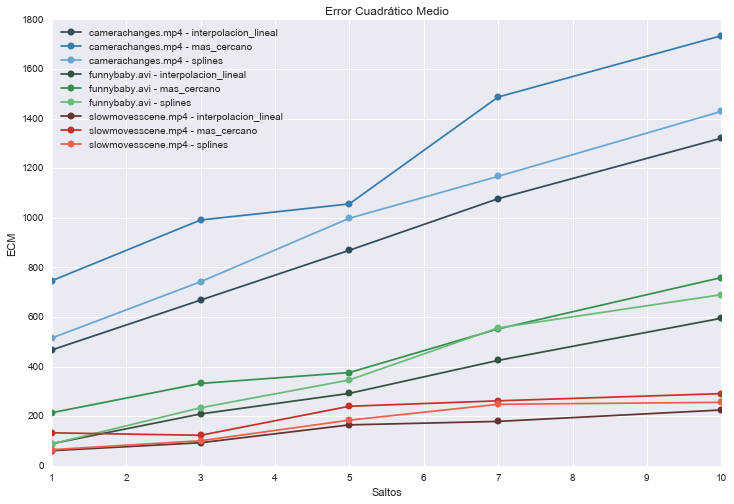
\includegraphics[width=.95\textwidth]{graficos/ecm.png}
\end{figure}

\vspace{-2em}
\begin{tiny}Este gr\'afico puede ser dificil de interpretar en blanco y negro\end{tiny}
\vspace{2em}

Este gr\'afico cementa la hipotesis de que \textit{camerachanges.avi}, que tiene
muchos cambios de c\'amara lo que hace que sea dificil predecir el valor de dos
pixeles cuando se pone en le c\'amara lenta tiene obviamente el mayor error. Por
otro lado, \textit{funnybaby.avi} y \textit{slowmoviescene.mp4} empiezan con un
\textbf{ECM} similar ya que ninguno de los dos tiene cambios bruscos, pero
cuando la cantidad de saltos aumenta el primer video empieza a tener un error
mucho mayor, ya que los cambios en el video dependientes del movimiento de la
cabeza del beb\'e \footnote{este es un beb\'e especialmente cabez\'on en comparaci\'on al
tama\~no del video} son mucho m\'as bruscos que los del video anterior.

Para comparar los m\'etodos, podemos ver el gr\'afico anterior y uno que tenga
solamente los valores para \textit{funnybaby.avi}

\begin{figure}[H]
\centering
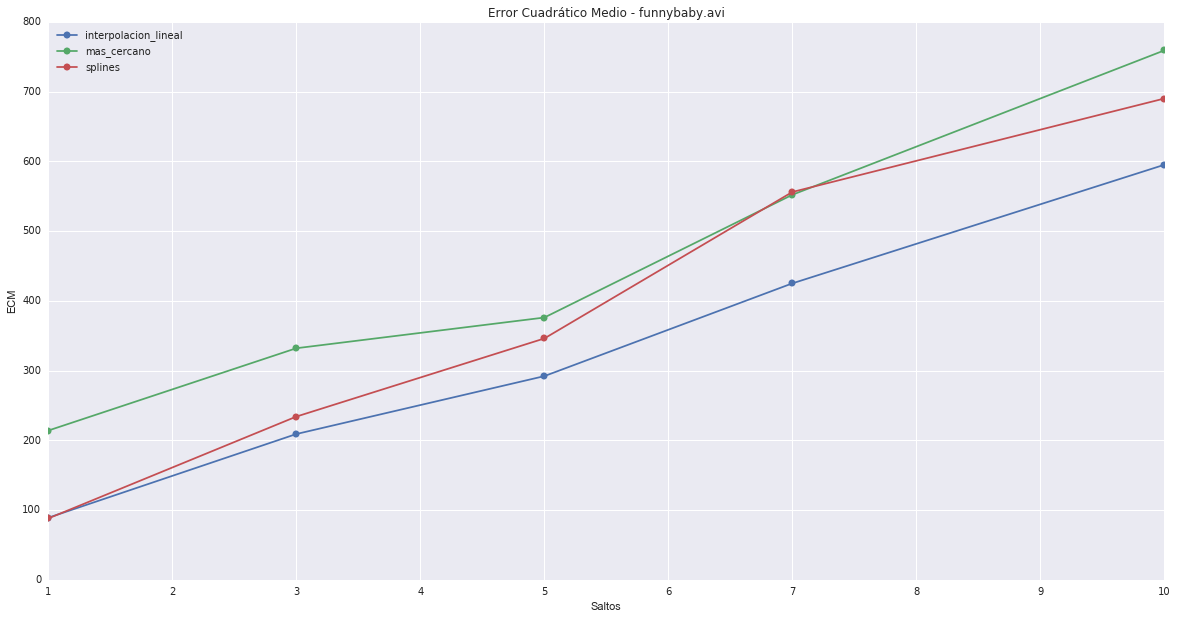
\includegraphics[width=.95\textwidth]{graficos/ecm_funnybaby.png}
\end{figure}

Como podemos ver, en todos los videos el m\'etodo de \textbf{interpolaci\'on
lineal} es el que genera menores errores, inclusive menos que el de splines.

El an\'alisis por \textbf{PSNR} da un resultado similar al de \textbf{ECM}, ya
que los dos m\'etodos est\'an inversamente relacionados. Sin embargo, se nota
con m\'as claridad que cuando hay pocos saltos el resultado puede ser altamente
diferente.

\begin{figure}[H]
\centering
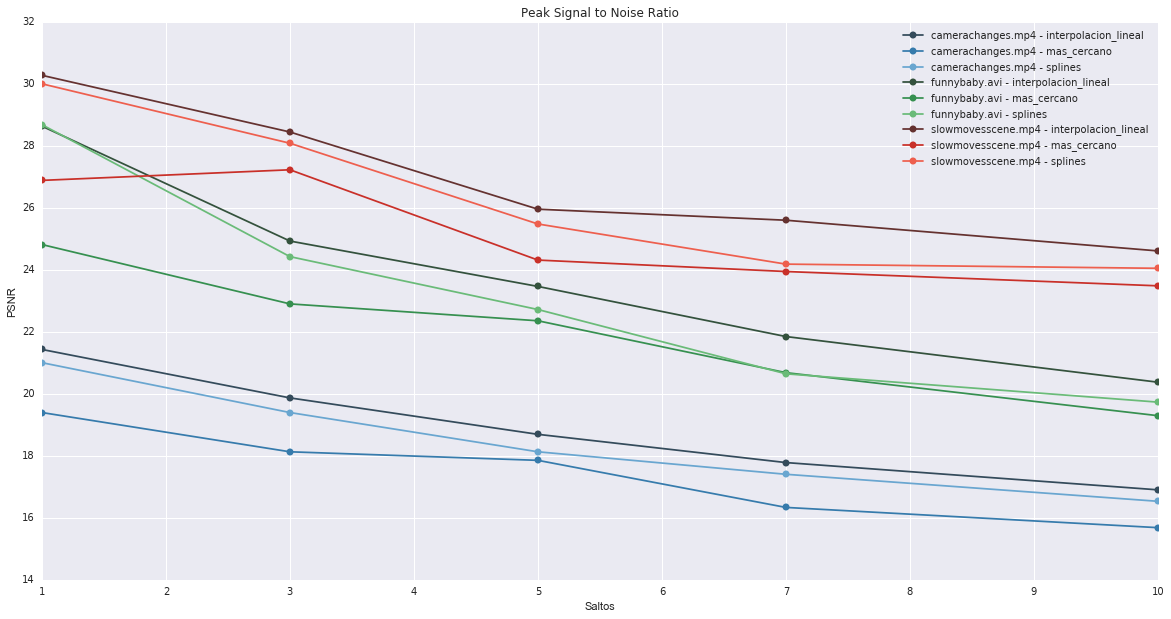
\includegraphics[width=.95\textwidth]{graficos/psnr.png}
\end{figure}
\vspace{-2em}
\begin{tiny}Este gr\'afico puede ser dificil de interpretar en blanco y negro\end{tiny}
\vspace{2em}

\subsection{An\'alisis de la velocidad de los algoritmos}

\subsubsection{Comparaci\'on entre m\'etodos}

Todos los m\'etodos que usamos en la c\'amara lenta se aplican individualmente a
cada pixel, por lo tanto la complejidad temporal de los m\'etodos debe ser de la
forma $ \mathbb{O}(h \cdot w \cdot f^{(m)}(c_1)) $, con $h$ y $w$ alto y ancho del
video, respectivamente, $c_1$ la cantidad de frames del video final, y $f^{(m)}$
alguna funci\'on que depende del m\'etodo.

Como adem\'as ninguno de los tiempos de corrida de los m\'etodos cambia
dependiendo del valor de los pixeles \footnote{descontando el tiempo del
condicional cuando se pasa del rango de pixeles, que deber\'ia ser negligible},
una buena manera de medir la eficiencia de los m\'etodos es aplicandolos al
mismo video con diferente salto $s$ (ya que, para un $c_0$ fijo, tiene una
correlaci\'on lineal con $c_1$). Para este caso decidimos usar
\textit{baby.avi}.

Por cada m\'etodo, medimos la eficiencia de ese m\'etodo tomando el tiempo que
tarda en aplicar la c\'amara lenta a \textit{baby.avi} con diferentes 

\begin{figure}[H]
\centering
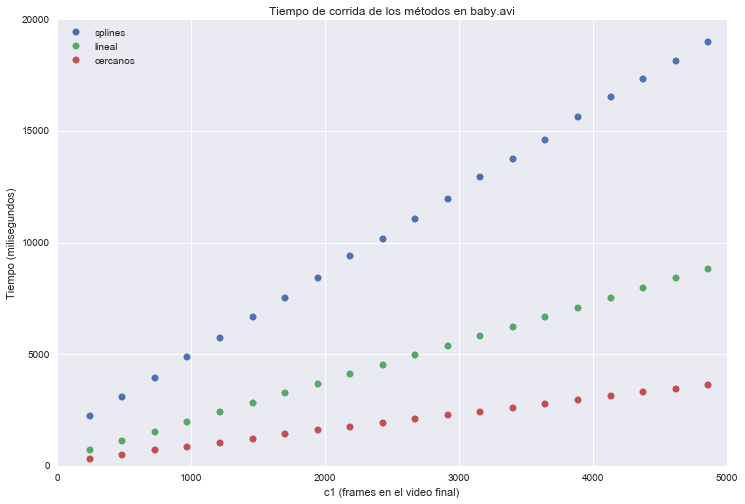
\includegraphics[width=.95\textwidth]{graficos/tiempo_baby.png}
\end{figure}

El gr\'afico da resultados previsibles: el tiempo de corrida del m\'etodo de los
splines es mayor que el de la interpolaci\'on lineal, que es mayor al de los
vecinos m\'as cercanos. Esto se debe a que, como explicado en el desarrollo,
el m\'etodo de los vecinos m\'as cercanos simplemente compia un valor de un
frame a otro y el de interpolaci\'on lineal hace una cuenta simple en punto
flotante, mientras que el de splines resuelve un sistema de $c_1$ ecuaciones.

Otra conclusi\'on que se puede sacar de este gr\'afico es que los tres m\'etodos
tiene complejidad temporal lineal. La raz\'on de esto es trivial en el caso de los
vecinos m\'as cercanos y el de la interpolaci\'on lineal, mientras que en el
caso de los splines nos aprovechamos que la matriz del sistema a resolver es
banda, lo que nos permite resolverlo en complejidad $\mathbb{O}(c_1)$ en vez de
la usual $\mathbb{O}(c_1^3)$.

\subsubsection{Reset en el m\'etodo de los splines}

Otro par\'ametro que puede tomar el \'ultimo m\'etodo, como est\'a explicado en
el desarrollo, es $r$, el ``reset'' del algoritmo. Esto indica que, en vez de
crear un sistema de ecuaciones para todos los puntos temporales en cada pixel,
va a crear sistemas de ecuaciones de tama\~no $r$ \footnote{posiblemente el
\'ultimo sea un poco m\'as grande}, y resolver cada sistema por separado.
Seg\'un nuestra hipotesis, esto deber\'ia resultar en un m\'etodo m\'as r\'apido
pero menos efectivo.

Para probarlo, dado que para probarlo eficientemente debemos hacerlo en videos
con un alto $c_1$, aprovechamos la propiedad de que el algoritmo funciona en
cada pixel por separado y creamos un video de tama\~no $1 \times 1$, con $c_0 =
100000$. De esta manera, podemos hacer las mismas pruebas m\'as r\'apido.

\begin{figure}[H]
\centering
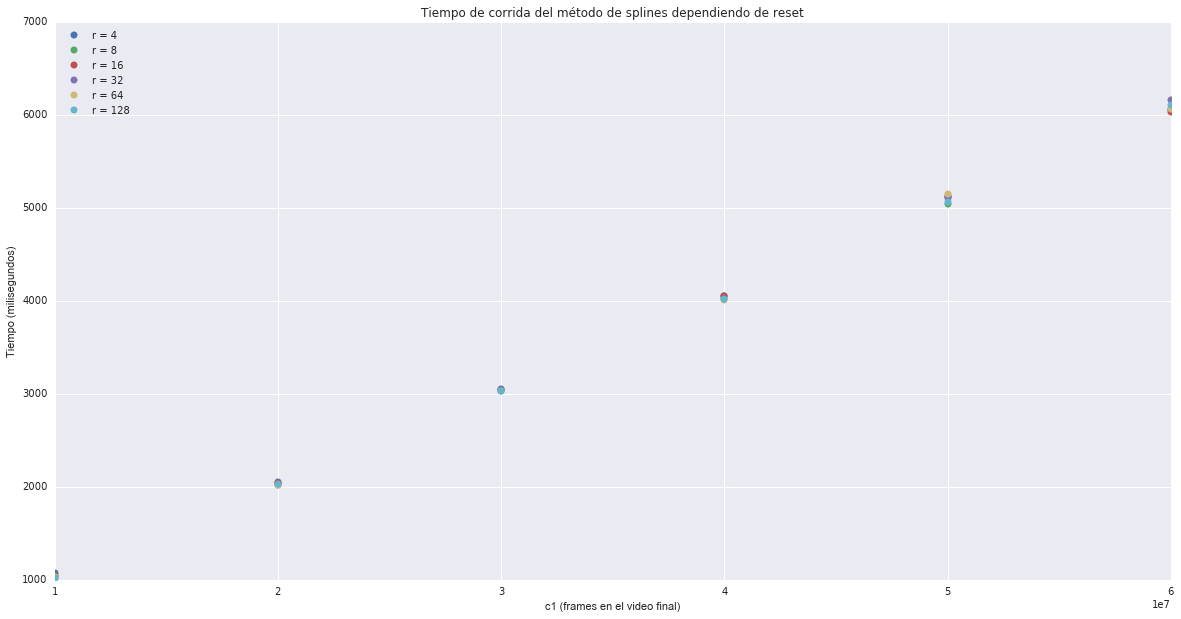
\includegraphics[width=.95\textwidth]{graficos/tiempo_reset.png}
\end{figure}

Por los resultados de los tiempos de la corrida podemos ver que nuestra
hip\'otesis es falsa. Al parecer, el algoritmo lineal para resolver el sistema
de ecuaciones con la matriz banda es lo suficientemente eficiente como para que
las ganancias de trabajar con matrices m\'as chicas sean negiglibles cuando se
les suma el costo de preparar y juntar las soluciones.
